\pagestyle{fancy}
\fancyhead[l]{\autorUO}
\fancyfoot[l]{\asignaturaAbbr}
\fancyfoot[r]{\fecha}

\section{Fases 2 y 3} \label{sec:4}
En esta sección se presentan los resultados obtenidos en la Fase 2 y Fase 3 del experimento. Para ello, se han tomado los tiempos de 
ejecución de la multiplicación de matrices en ambas fases utilizando los siguientes tamaños de 
matrices: $2,\ 4,\ 8,\ 16,\ 32,\ 64,\ 128,\ 256,\ 398,\ 512,\ 636,\ 774,\ 892,\ 1024,\ 1152,\ 1280,\ 1408 \ y \ 1536$. 
En el caso del algoritmo de \zorder, se ha ejecutado con todos los tamaños de bloque posibles para cada tamaño de matriz.
Todos los productos se han repetido un total de $8$ iteraciones, y se ha tomado el tiempo medio de ejecución.

El objetivo principal de esta sección es comparar cómo afecta en los tiempos de ejecución la creación y el manejo de las matrices 
en \python\ o en \C, ya que, en ambos casos, el producto de matrices se realiza en este último lenguaje.

\subsection{\rowmajor\ y \colmajor} \label{sec:4.1}
En la \autoref{fig:3} se presentan los resultados obtenidos para \rowmajor\ y \colmajor\ en ambas fases.

\begin{figure}[h]
    \centering
    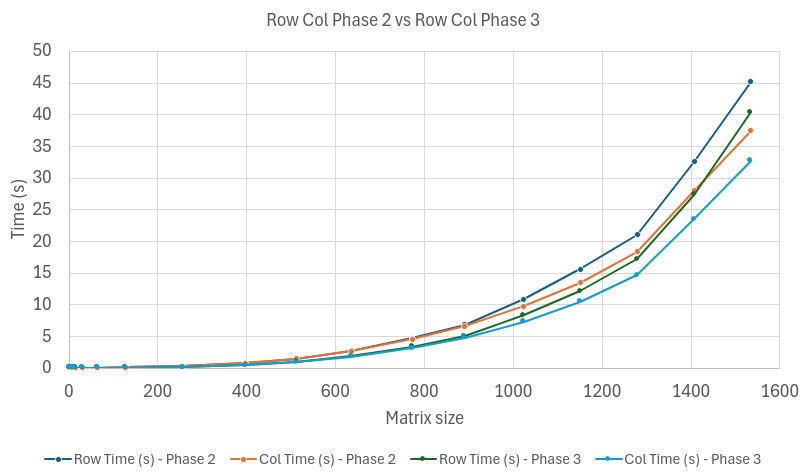
\includegraphics[width=0.55\textwidth]{img/3.png}
    \caption{Tiempos de ejecución de \rowmajor\ y \colmajor\ en Fase 2 y Fase 3}
    \label{fig:3}
\end{figure}

En cuanto a progresión, se observa un crecimiento exponencial prácticamente similar en ambos casos, con la pequeña particularidad 
de que los tiempos obtenidos en la Fase 3 son ligeramente más rápidos que los de la Fase 2. Esto tiene sentido y cumple el 
comportamiento esperado, ya que en la Fase 2 se crean las matrices en \python\ y posteriormente se pasan a \C\ para su
multiplicación, mientras que en la Fase 3 se crean las matrices directamente en \C\ y se multiplican en este mismo lenguaje. \\
En la \autoref{tab:2} se presentan parte de los tiempos de ejecución obtenidos en ambas fases.

\renewcommand{\arraystretch}{1.1}
\begin{table}[h]
    \centering
    \begin{tabular}{|c|c|c|c|c|}
        \hline
        & \multicolumn{2}{|c|}{Phase 2} & \multicolumn{2}{c|}{Phase 3} \\ \hline
        Matrix size & \rowmajor\ (s) & \colmajor\ (s) & \rowmajor\ (s) & \colmajor\ (s) \\ \hline
        $774 \times 774$ & $4.620579$ & $4.460339$ & $3.318547$ & $3.097386$ \\
        $892 \times 892$ & $6.753538$ & $6.553215$ & $4.989206$ & $4.763061$ \\
        $1024 \times 1024$ & $10.842022$ & $9.681300$ & $8.309243$ & $7.257873$ \\
        $1280 \times 1280$ & $20.950864$ & $18.301773$ & $17.14470$ & $14.620171$ \\
        $1408 \times 1408$ & $32.527939$ & $27.930434$ & $27.32356$ & $23.420535$ \\
        $1536 \times 1536$ & $45.130261$ & $37.390848$ & $40.28853$ & $32.658900$ \\ \hline
    \end{tabular}
    \caption{Tiempos de ejecución de \rowmajor\ y \colmajor\ en Fase 2 y Fase 3}
    \label{tab:3}
\end{table}
\renewcommand{\arraystretch}{1.0}
\newpage

Con esta representación numérica, la diferencia de tiempos entre ambas fases es mucho más notable. De hecho, esta diferencia 
aumenta conforme aumenta el tamaño de la matriz, lo cual es lógico, ya que la reserva de memoria y el manejo 
de matrices mayores consume más tiempo. \\
En la \autoref{fig:4} se presenta esta diferencia de tiempos entre \rowmajor\ y \colmajor\ en ambas fases.

\begin{figure}[h]
    \centering
    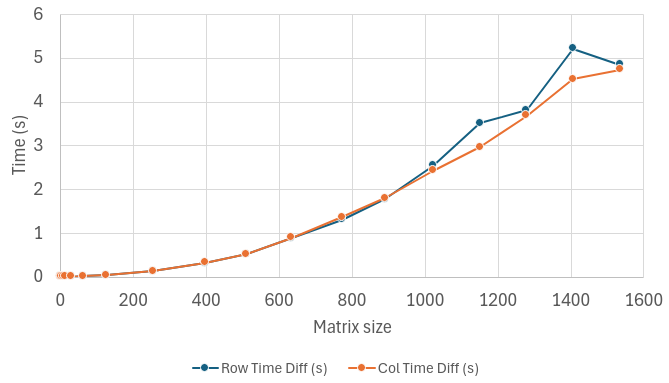
\includegraphics[width=0.55\textwidth]{img/4.png}
    \caption{Diferencia de tiempos de ejecución entre \rowmajor\ y \colmajor\ en Fase 2 y Fase 3}
    \label{fig:4}
\end{figure}

Se puede observar una tendencia exponencial en la diferencia de tiempos conforme el tamaño de la matriz aumenta, si bien es cierto 
que es más clara en el caso de \colmajor\ que en el de \rowmajor. Esta pequeña variación en la tendencia exponencial en el caso de \rowmajor\ 
se asocia con variaciones en el contexto operativo del sistema durante la toma de tiempos.

\subsection{\zorder} \label{sec:4.2}
A continuación se analizan los resultados obtenidos para el algoritmo \zorder\ en Fase 2 y Fase 3. La tendencia de los tiempos de 
ejecución en ambas es muy similar, con la salvedad de que en la Fase 3 los tiempos son más rápidos. En la 
\autoref{fig:5} se presentan los resultados obtenidos para el tamaño de matriz $1536 \times 1536$.

\begin{figure}[h]
    \centering
    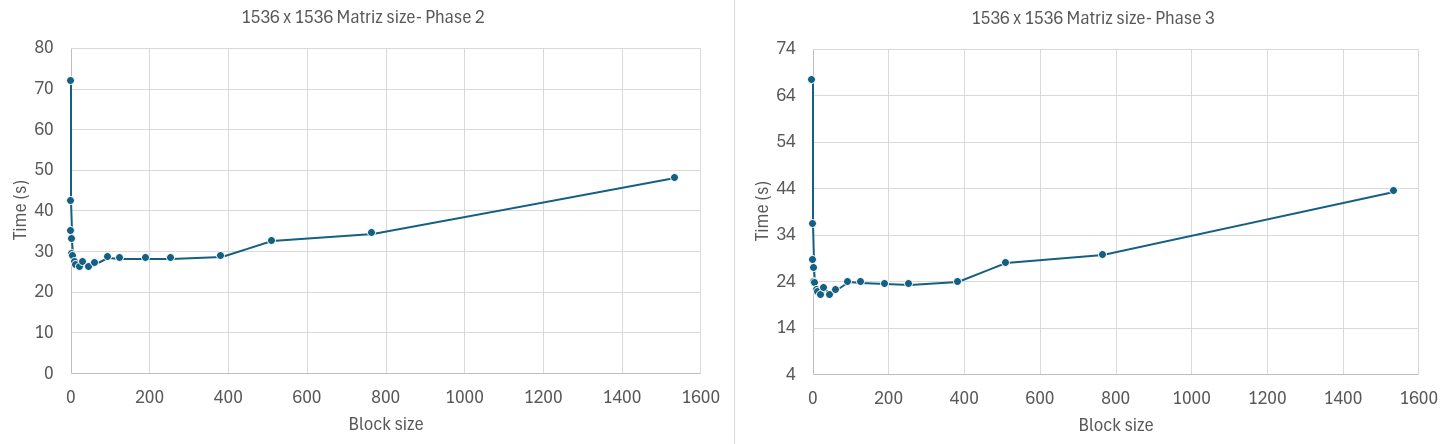
\includegraphics[width=0.98\textwidth]{img/5.png}
    \caption{Tiempos de ejecución de \zorder\ en Fase 2 y Fase 3 ($N = 1536$)}
    \label{fig:5}
\end{figure}

Como se puede observar, la tendencia es prácticamente la misma para los diferentes tamaños de bloque. Esto sucede para cada 
tamaño de matriz y es así porque en ambos casos el producto de matrices se realiza en \C. Por lo tanto, se pasará a estudiar 
la diferencia de tiempos debida al manejo de matrices en \python\ o en \C. 
\newpage

En la \autoref{fig:6} se representa el mejor tiempo de ejecución obtenido con \zorder\ (con el tamaño de bloque óptimo) para 
cada tamaño de matriz en ambas fases.

\begin{figure}[h]
    \centering
    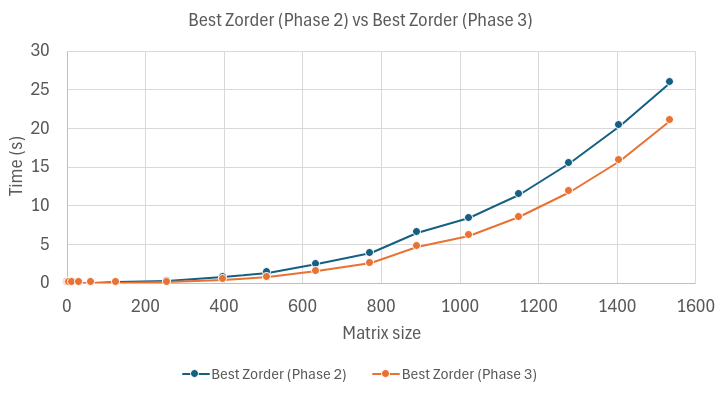
\includegraphics[width=0.55\textwidth]{img/6.png}
    \caption{Diferencia de tiempos de ejecución entre \zorder\ en Fase 2 y Fase 3}
    \label{fig:6}
\end{figure}

La tendencia de ambas funciones es la misma, haciéndose notar la diferencia de rendimiento que supone manejar las matrices 
en \C\ (Fase 3) respecto a \python\ (Fase 2). Esta diferencia de tiempos se representa en la \autoref{fig:7}.

\begin{figure}[h]
    \centering
    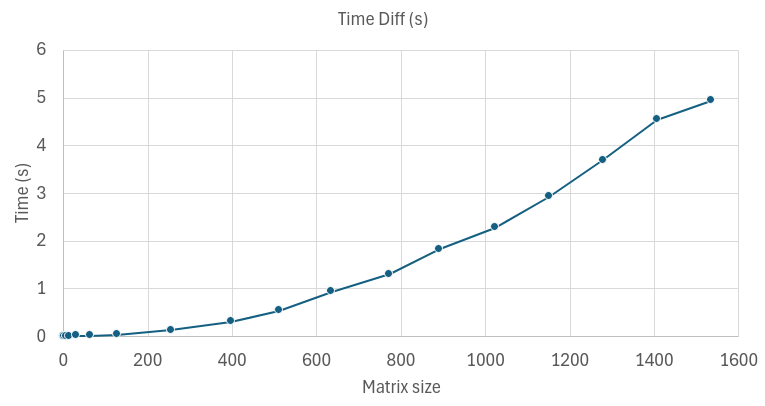
\includegraphics[width=0.55\textwidth]{img/7.png}
    \caption{Diferencia de tiempos de ejecución de \zorder\ en Fase 2 y Fase 3}
    \label{fig:7}
\end{figure}

Se obtiene una función con tendencia exponencial conforme el tamaño de matriz aumenta, tal y como sucedía en la 
\autoref{fig:4} para \rowmajor\ y \colmajor. Por lo tanto, como ya se esperaba, la diferencia de rendimiento entre 
ambas fases con cada uno de los algoritmos probados se debe única y exclusivamente a cómo se manejan las matrices, 
siendo \C\ el lenguaje más eficiente para este tipo de operaciones.

